\clearpage
\appendix
\markright{Appendix}

\section*{Appendix}
\addcontentsline{toc}{section}{Appendix}

This appendix contains the complete codebase for the problems solved in this midterm. All implementations are written in Julia and developed from scratch without using built-in numerical solver shortcuts.

% =====================
% Problem 3 Appendix
% =====================
\subsection*{Problem 3: LU and Cholesky Factorization}
\addcontentsline{toc}{subsection}{Problem 3: LU and Cholesky Factorization}
\label{appendix:p03-code}

The following figures show the Julia implementation for Problem 3.

\begin{figure}[H]
    \centering
    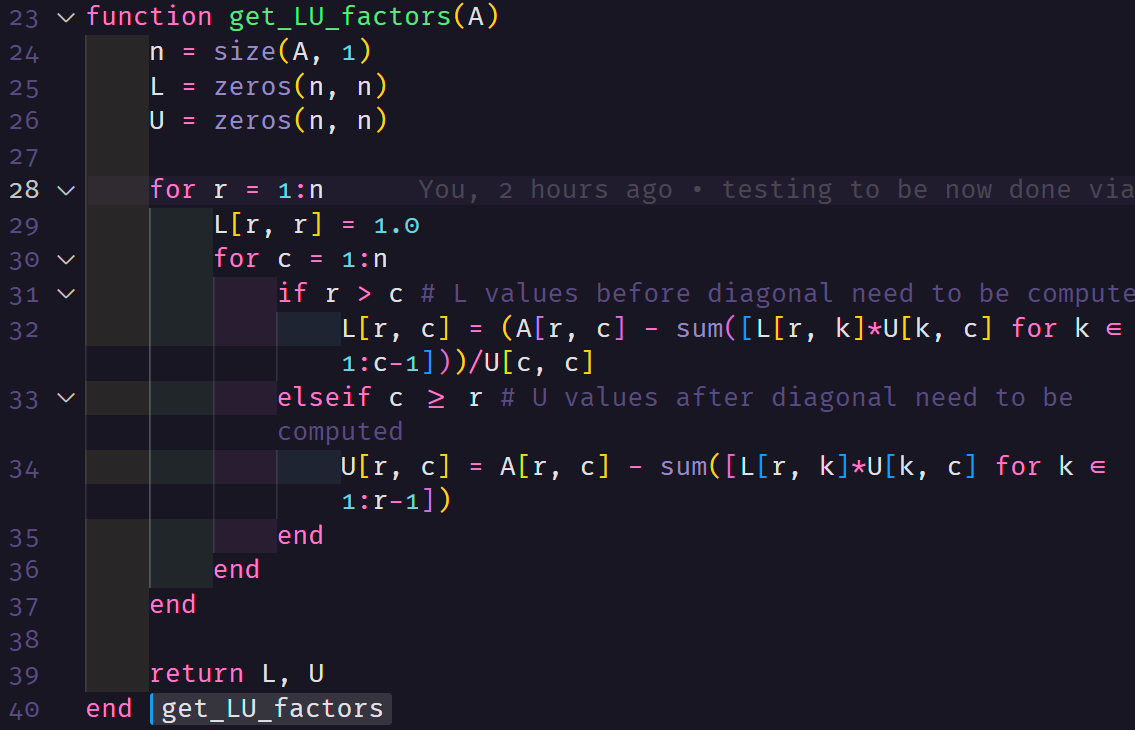
\includegraphics[width=0.95\textwidth]{figures/p03-codebase-1-get-LU-factors.png}
    \caption{LU Factorization function: \texttt{get\_LU\_factors(A)} implements the Doolittle algorithm with unit lower triangular matrix $\mathbf{L}$.}
    \label{fig:p03-code-lu}
\end{figure}

\begin{figure}[H]
    \centering
    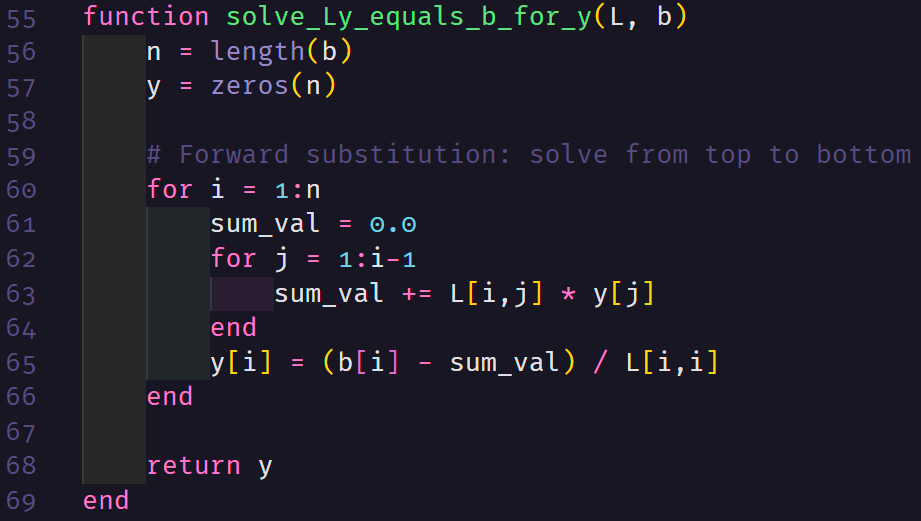
\includegraphics[width=0.95\textwidth]{figures/p03-codebase-2-solve-Ly-equals-b-for-y.png}
    \caption{Forward substitution function: \texttt{solve\_Ly\_equals\_b\_for\_y(L, b)} solves the lower triangular system $\mathbf{Ly} = \mathbf{b}$ using simple nested loops.}
    \label{fig:p03-code-forward}
\end{figure}

\begin{figure}[H]
    \centering
    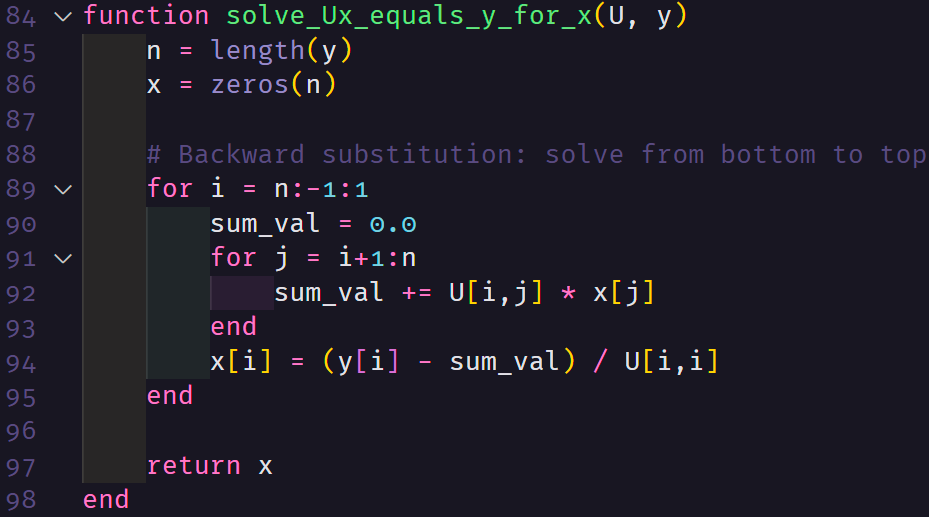
\includegraphics[width=0.95\textwidth]{figures/p03-codebase-3-solve-Ux-equals-y-for-x.png}
    \caption{Backward substitution function: \texttt{solve\_Ux\_equals\_y\_for\_x(U, y)} solves the upper triangular system $\mathbf{Ux} = \mathbf{y}$ using simple nested loops.}
    \label{fig:p03-code-backward}
\end{figure}

\begin{figure}[H]
    \centering
    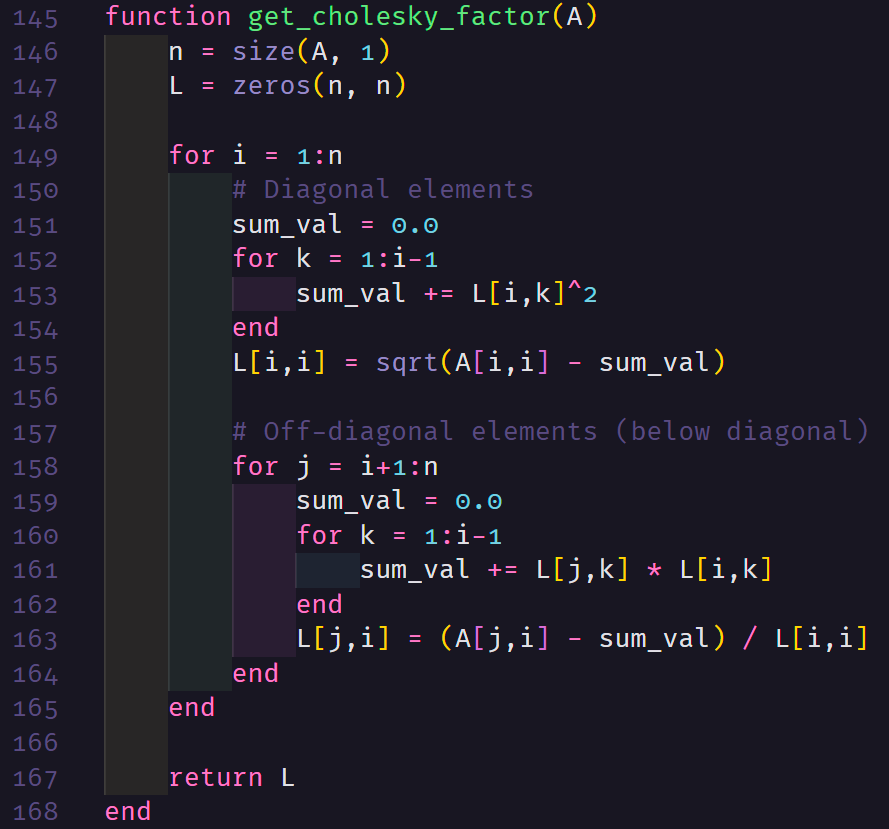
\includegraphics[width=0.95\textwidth]{figures/p03-codebase-4-get-cholesky-factors.png}
    \caption{Cholesky factorization function: \texttt{get\_cholesky\_factor(A)} implements the standard Cholesky algorithm for symmetric positive-definite matrices, computing $\mathbf{L}$ such that $\mathbf{A} = \mathbf{LL}^T$.}
    \label{fig:p03-code-cholesky}
\end{figure}

\begin{figure}[H]
    \centering
    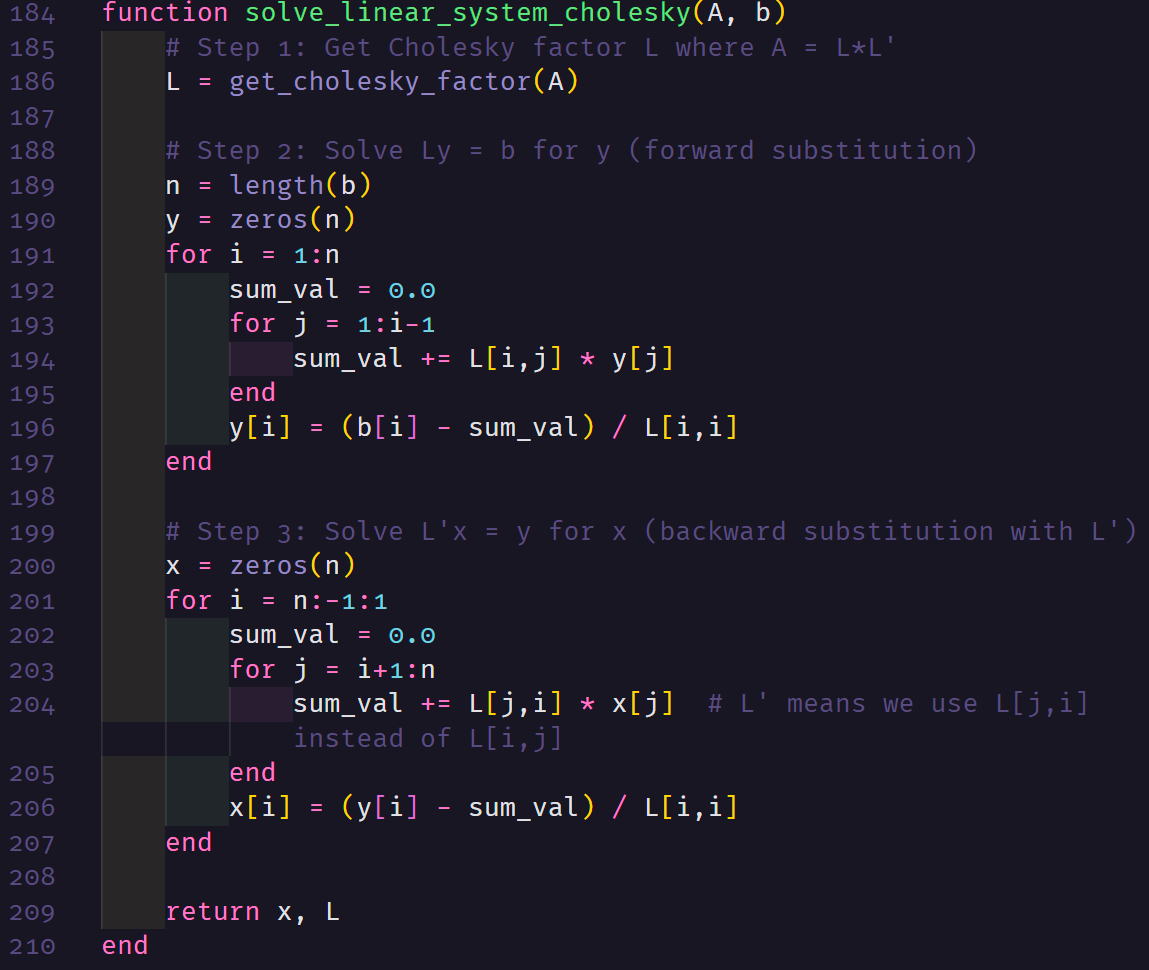
\includegraphics[width=0.95\textwidth]{figures/p03-codebase-5-solve-linear-system-cholesky.png}
    \caption{Complete Cholesky solver: \texttt{solve\_linear\_system\_cholesky(A, b)} combines Cholesky factorization with forward and backward substitution to solve $\mathbf{Ax} = \mathbf{b}$.}
    \label{fig:p03-code-cholesky-solver}
\end{figure}


% =====================
% Problem 4-2 Appendix
% =====================
\subsection*{Problem 4-2: FPI Iteration}
\addcontentsline{toc}{subsection}{Problem 4-2: FPI Iteration}

The following code implements the fixed point iteration (FPI) for Problem 4-2. The accompanying figure shows the FPI trajectory and convergence table as used in the main report (see \Cref{fig:p04-2-fpi-iterations-function}).

% \subsection*{Julia Code}
% \begin{lstlisting}[language=Julia]
% % Paste your FPI Julia code for p04-2 here
% \end{lstlisting}

\subsection*{FPI Iterations and Convergence}
\begin{figure}[H]
    \centering
    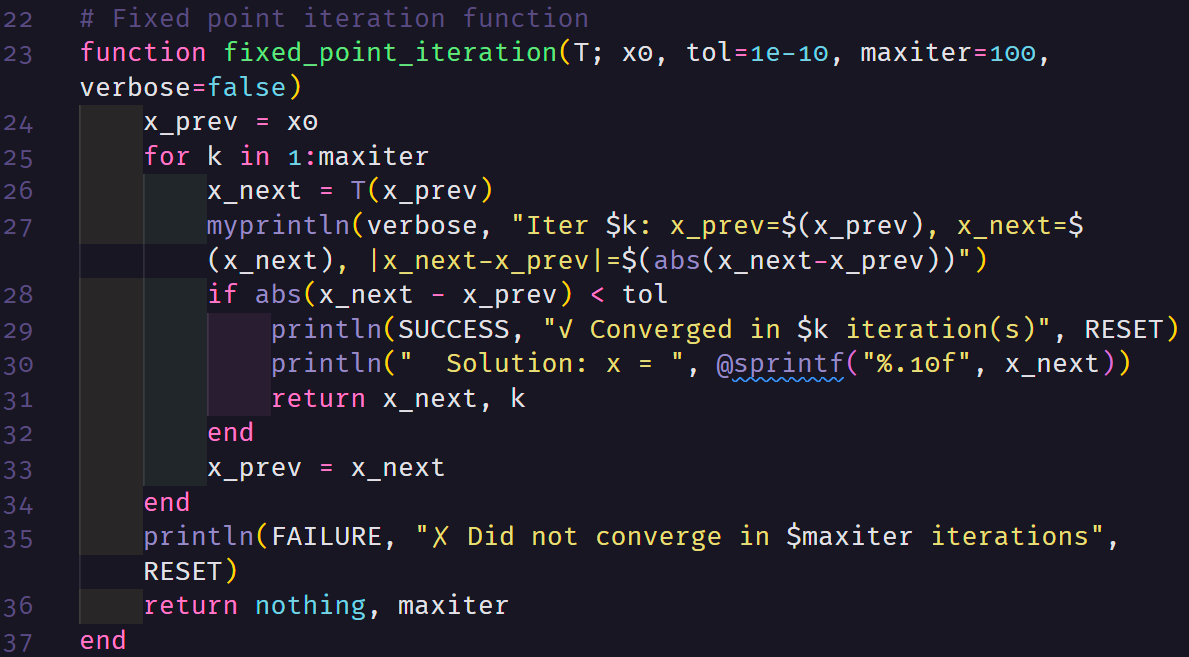
\includegraphics[width=0.85\textwidth]{figures/p04-2-fpi-iterations-function.png}
    \caption{FPI trajectory and convergence table for Problem 4-2. This illustrates the sequence of iterates and the error behavior discussed in the main text.}
    \label{fig:p04-2-fpi-iterations-function}
\end{figure}

% =====================
% Problem 4-4 Appendix
% =====================
\subsection*{Problem 4-4: Newton's Method}
\addcontentsline{toc}{subsection}{Problem 4-4: Newton's Method}

The following code implements Newton's method with FPI fallback for Problem 4-4. The figures below illustrate the method's logic and the convergence behavior referenced in the main report (see \Cref{fig:p04-4-newtons-method-with-fallback-function-part1,fig:p04-4-newtons-method-with-fallback-function-part2}).

% \subsection*{Julia Code}
% \begin{lstlisting}[language=Julia]
% % Paste your Newton/FPI fallback Julia code for p04-4 here
% \end{lstlisting}

\subsection*{Newton's Method with Fallback: Logic and Convergence}
\begin{figure}[H]
    \centering
    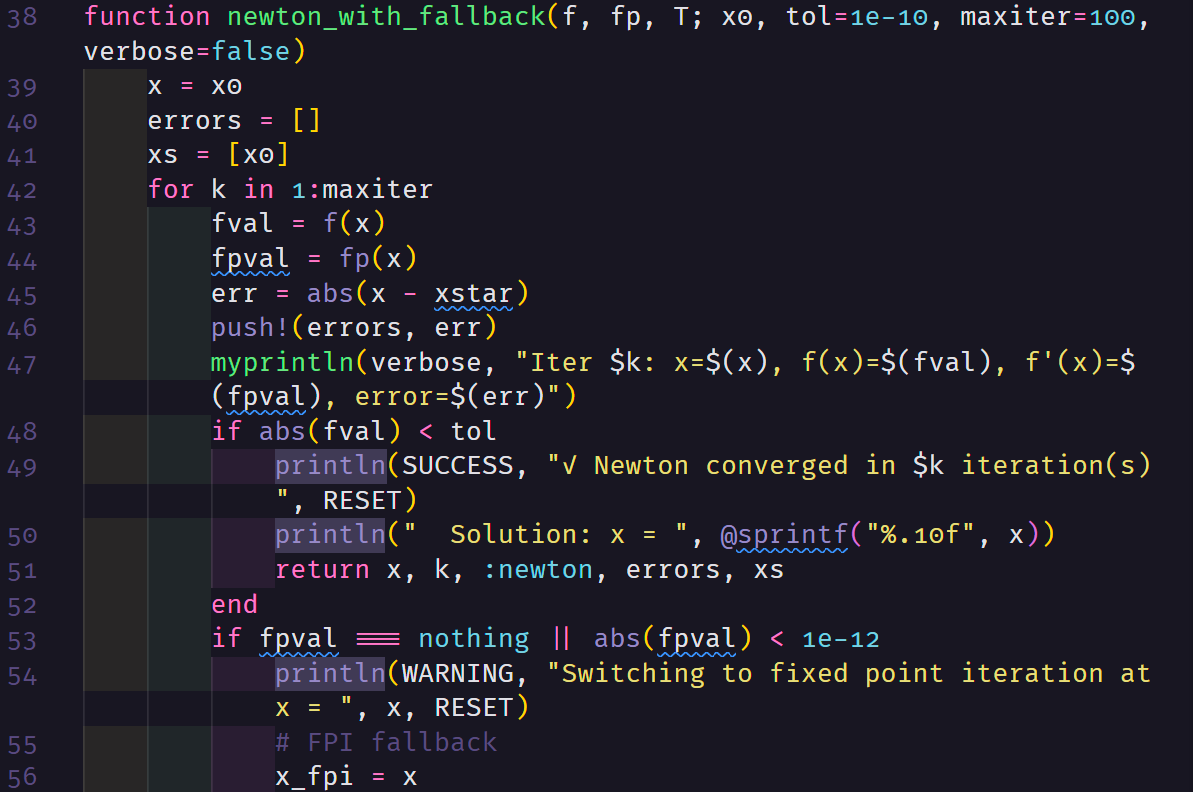
\includegraphics[width=0.85\textwidth]{figures/p04-4-newtons-method-with-fallback-function-part1.png}
    \caption{Newton's method with FPI fallback: logic and switching mechanism. This diagram clarifies the robust handling of non-differentiable points.}
    \label{fig:p04-4-newtons-method-with-fallback-function-part1}
\end{figure}

\begin{figure}[H]
    \centering
    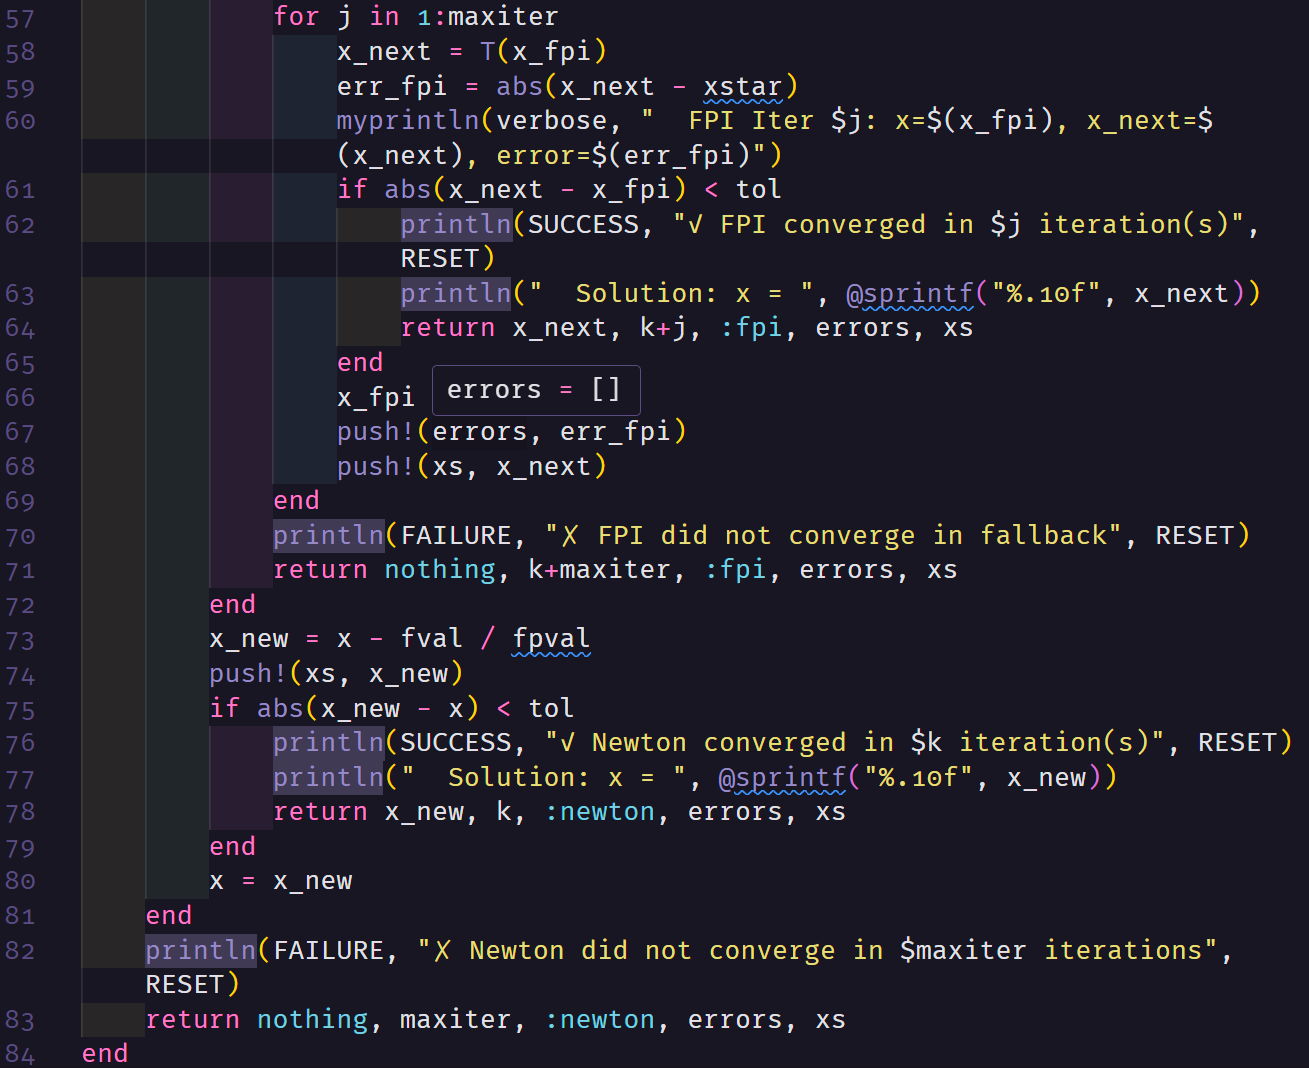
\includegraphics[width=0.85\textwidth]{figures/p04-4-newtons-method-with-fallback-function-part2.png}
    \caption{Newton's method with FPI fallback: convergence output and error table. This figure shows the rapid convergence and fallback behavior as discussed in the main text.}
    \label{fig:p04-4-newtons-method-with-fallback-function-part2}
\end{figure}

% =====================
% Problem 4-6 Appendix
% =====================
\subsection*{Problem 4-6: Alternative Error Control Strategy}
\addcontentsline{toc}{subsection}{Problem 4-6: Alternative Error Control Strategy}

The following code implements the alternative error control strategy for FPI in Problem 4-6. The figures below show the convergence analysis and the comparison of a posteriori and true errors, as referenced in the main report (see \Cref{fig:p04-6-alternative-error-control-strategy-function,fig:p04-6-aposteriori-vs-true-error-function}).

% \subsection*{Julia Code}
% \begin{lstlisting}[language=Julia]
% % Paste your FPI alternative error control Julia code for p04-6 here
% \end{lstlisting}

\subsection*{Alternative Error Control and Error Comparison}
\begin{figure}[H]
    \centering
    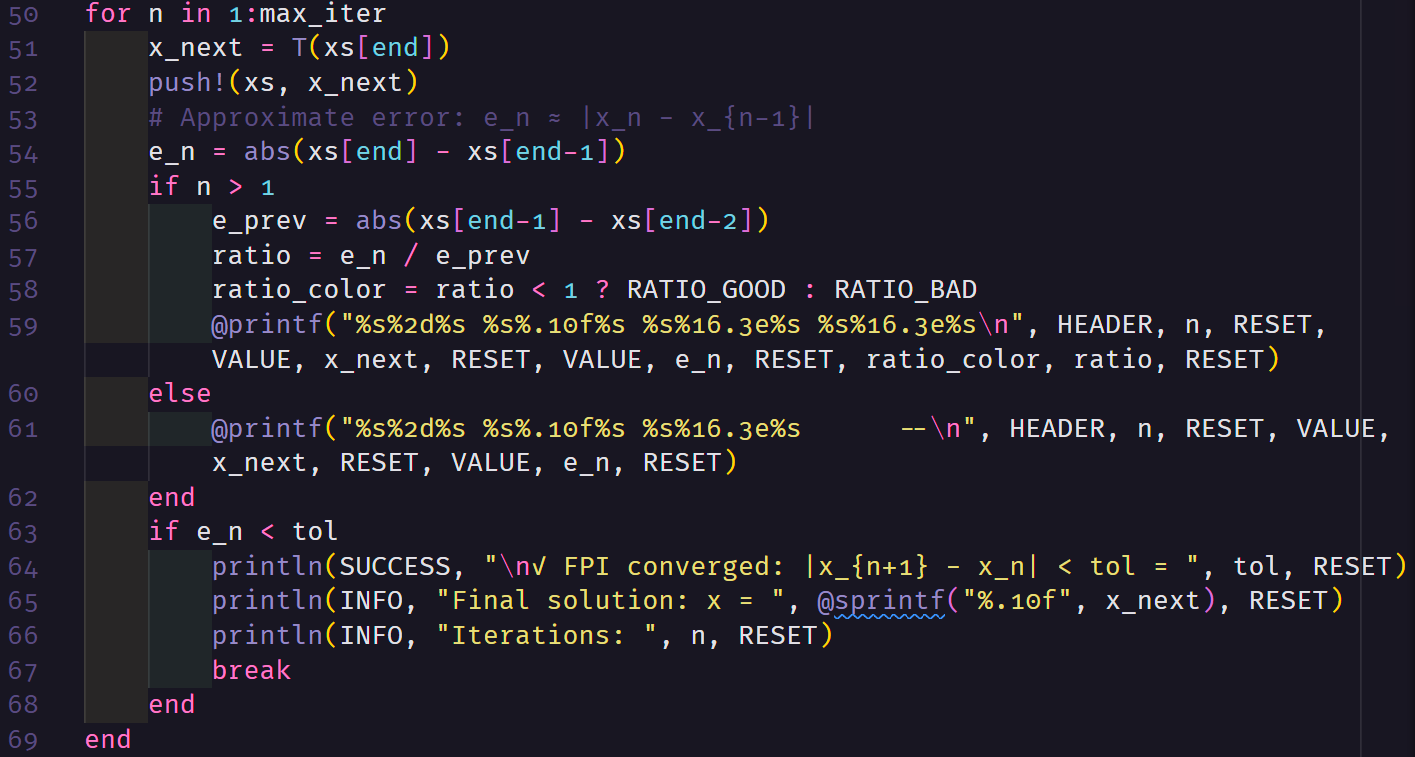
\includegraphics[width=0.85\textwidth]{figures/p04-6-alternative-error-control-strategy-function.png}
    \caption{Convergence analysis for the alternative error control strategy in Problem 4-6. This figure demonstrates the robust stopping and proximity criteria.}
    \label{fig:p04-6-alternative-error-control-strategy-function}
\end{figure}

\begin{figure}[H]
    \centering
    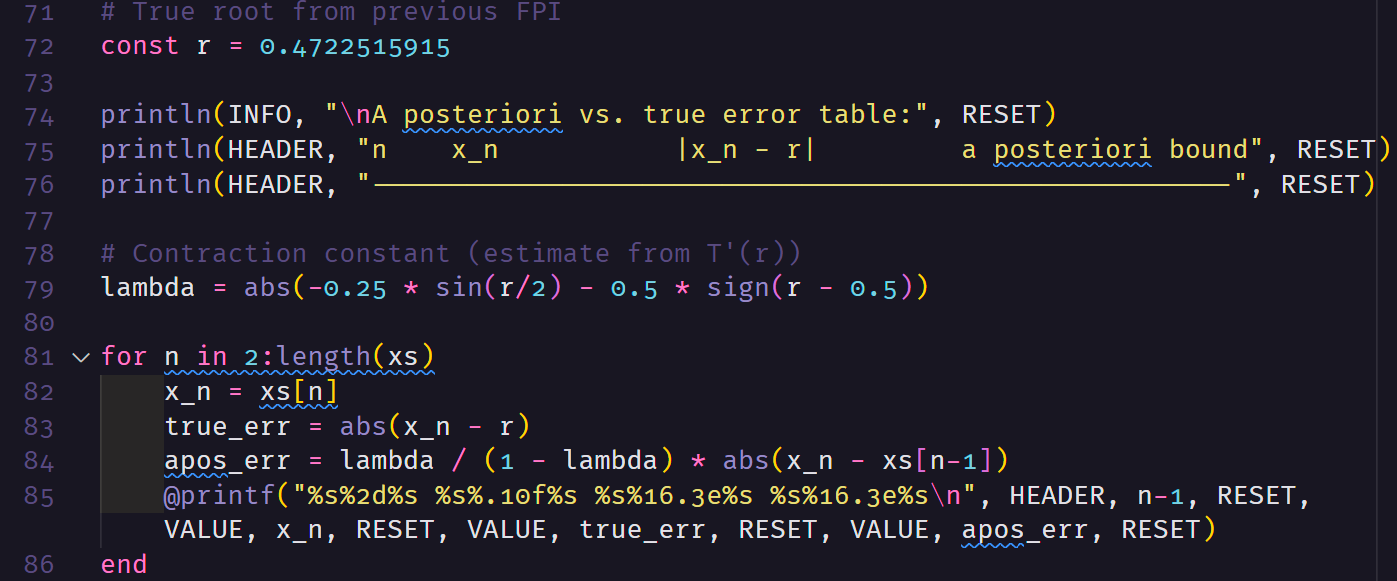
\includegraphics[width=0.85\textwidth]{figures/p04-6-aposteriori-vs-true-error-function.png}
    \caption{Comparison of a posteriori error bound and true error for each FPI iteration in Problem 4-6. This validates the reliability of the a posteriori estimate.}
    \label{fig:p04-6-aposteriori-vs-true-error-function}
\end{figure}

\subsection*{Problem 5-3: Ridders' Method Function}
\addcontentsline{toc}{subsection}{Problem 5-3: Ridders' Method Function}
\label{appendix:p05-3-code}

The following figures show the implementation of the Ridders' root-finding function, broken into logical parts. The bisection method is not shown here, as it was implemented in Homework 1 and is a subset of Ridders' approach.

\begin{figure}[H]
    \centering
    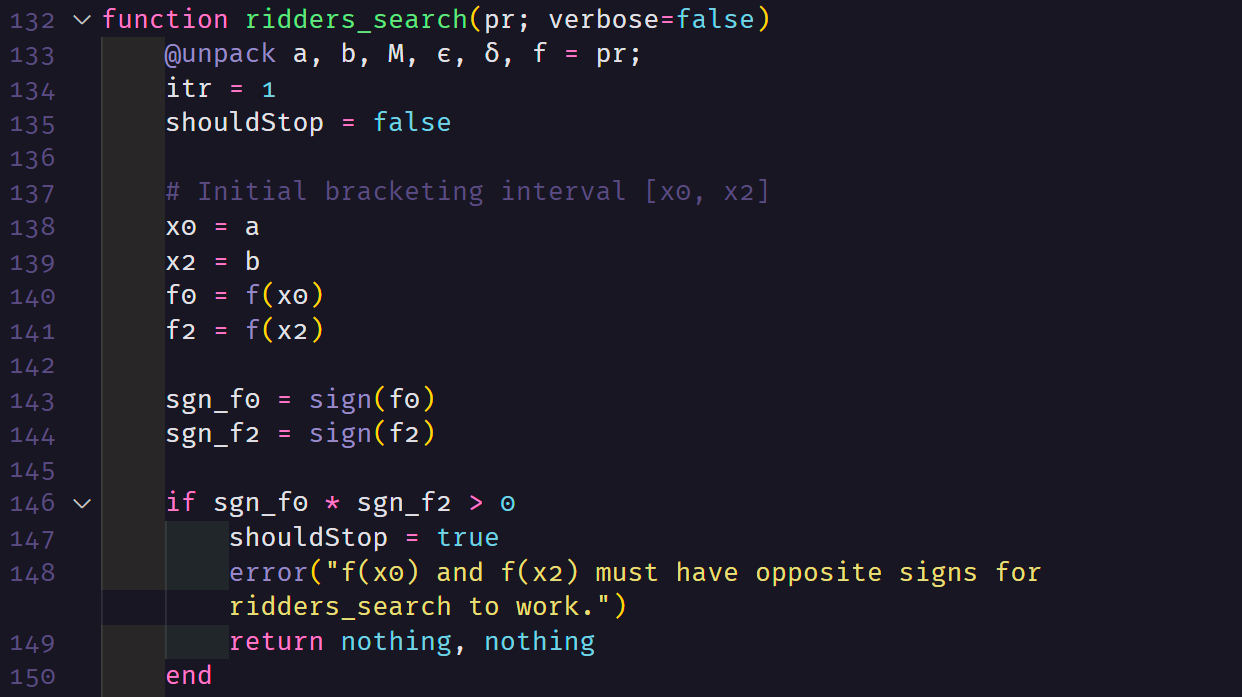
\includegraphics[width=0.95\textwidth]{figures/p05-3-codebase-1-ridders-search-part1.png}
    \caption{Ridders' function (part 1): Initial setup and input checks.}
\end{figure}

\begin{figure}[H]
    \centering
    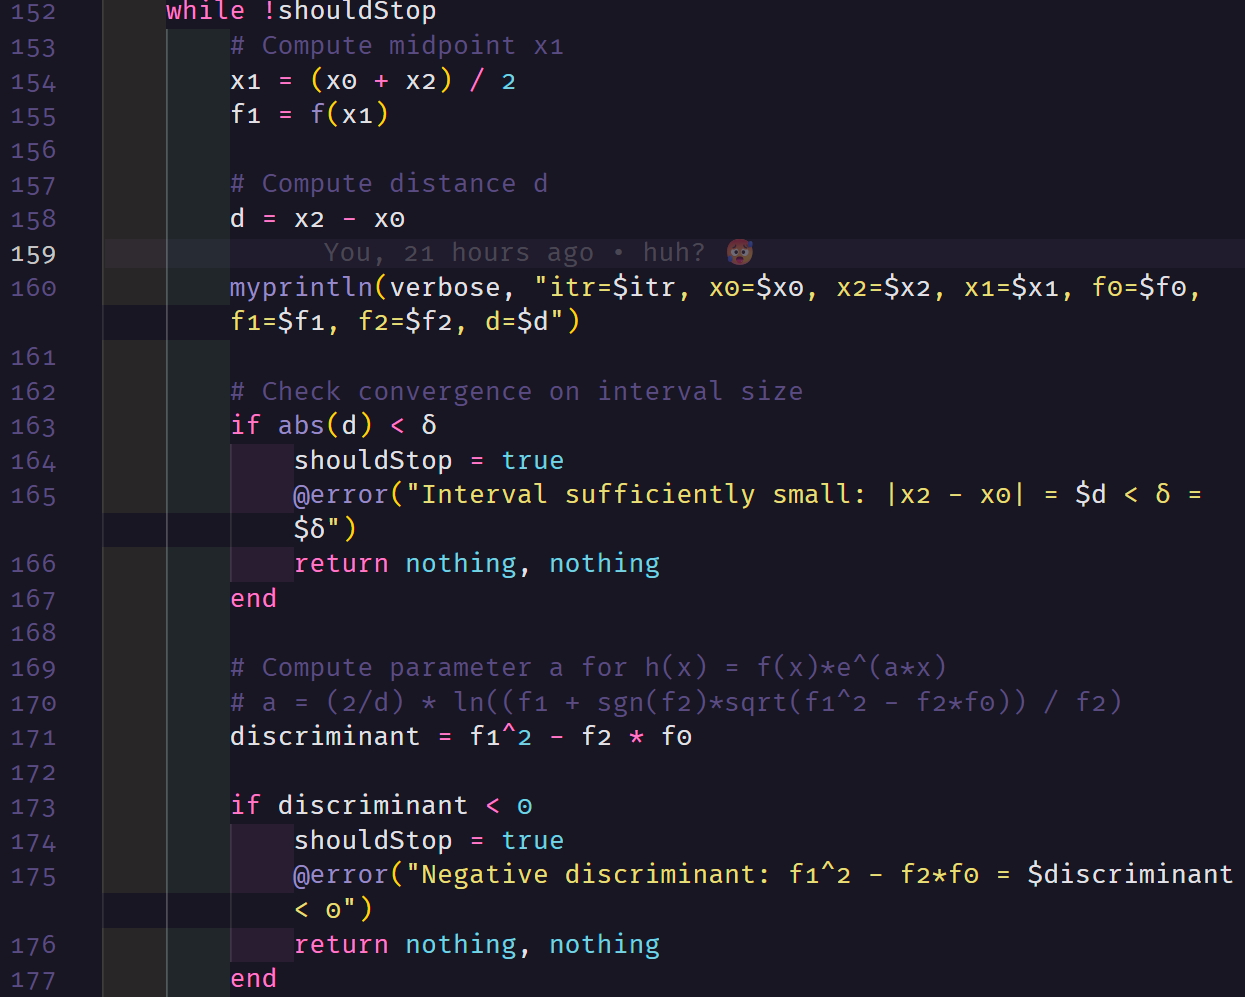
\includegraphics[width=0.95\textwidth]{figures/p05-3-codebase-2-ridders-search-part2.png}
    \caption{Ridders' function (part 2): Main loop and interval update.}
\end{figure}

\begin{figure}[H]
    \centering
    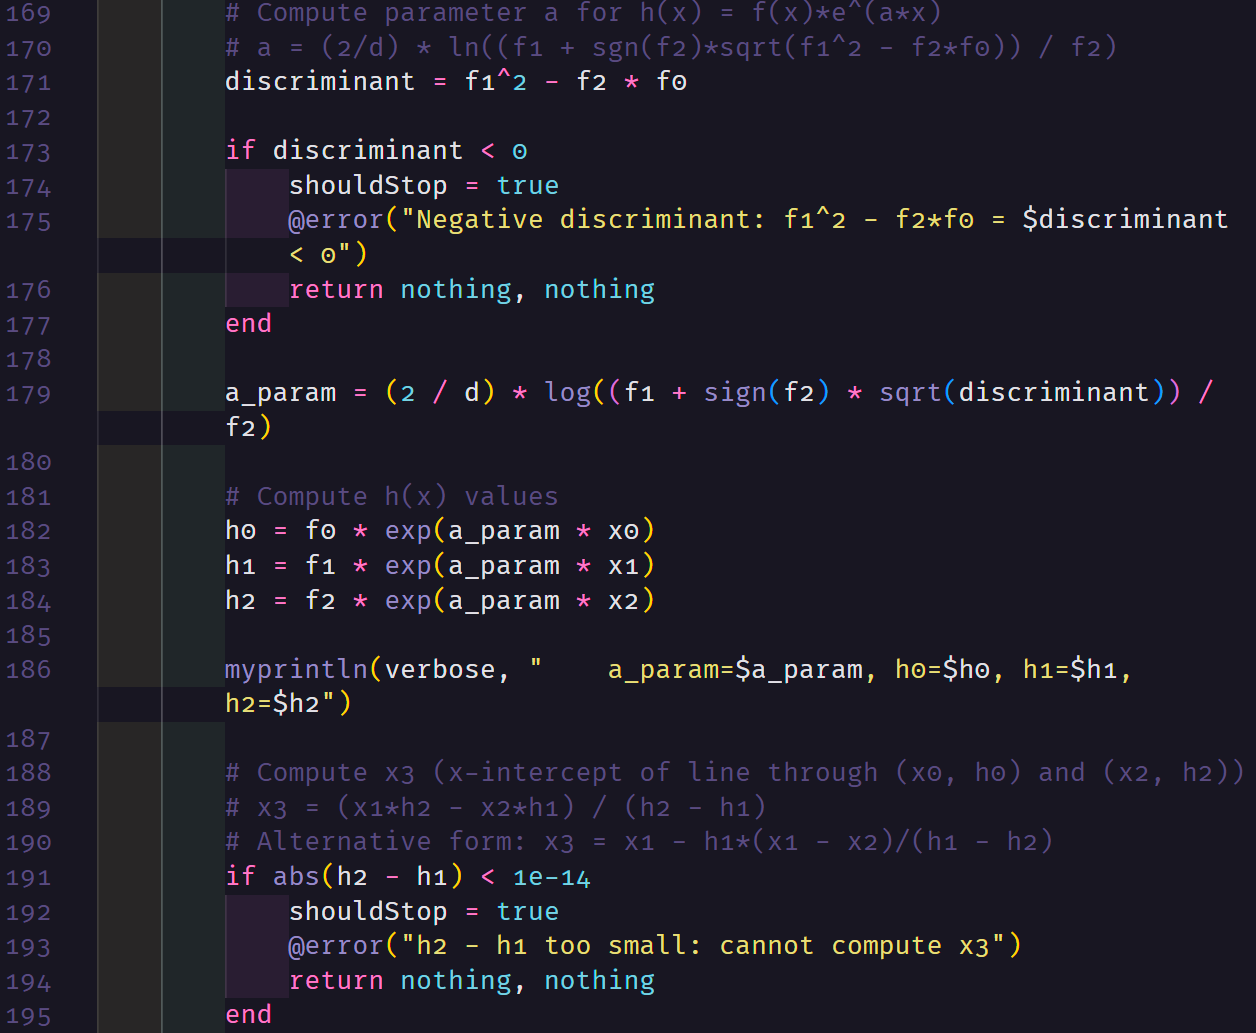
\includegraphics[width=0.95\textwidth]{figures/p05-3-codebase-3-ridders-search-part3.png}
    \caption{Ridders' function (part 3): Compute midpoint and evaluate function.}
\end{figure}

\begin{figure}[H]
    \centering
    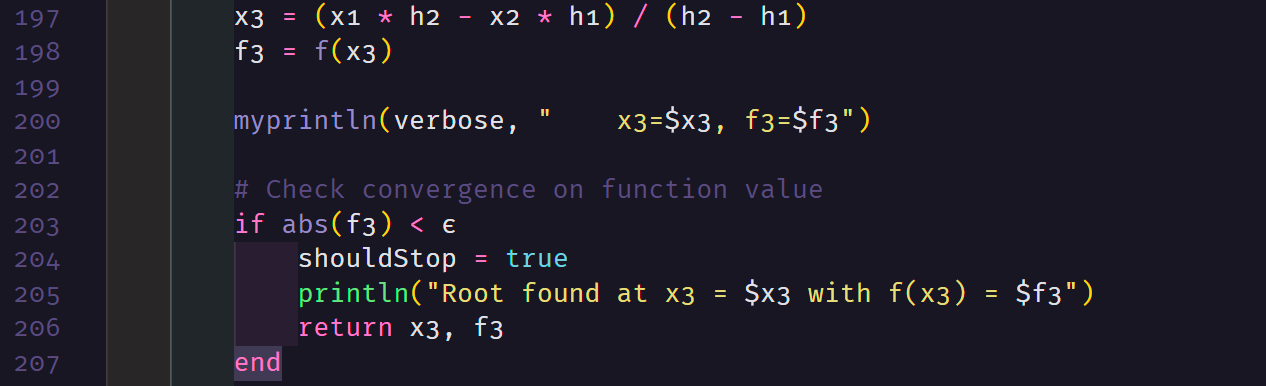
\includegraphics[width=0.95\textwidth]{figures/p05-3-codebase-4-ridders-search-part4.png}
    \caption{Ridders' function (part 4): Ridders' formula and root estimate.}
\end{figure}

\begin{figure}[H]
    \centering
    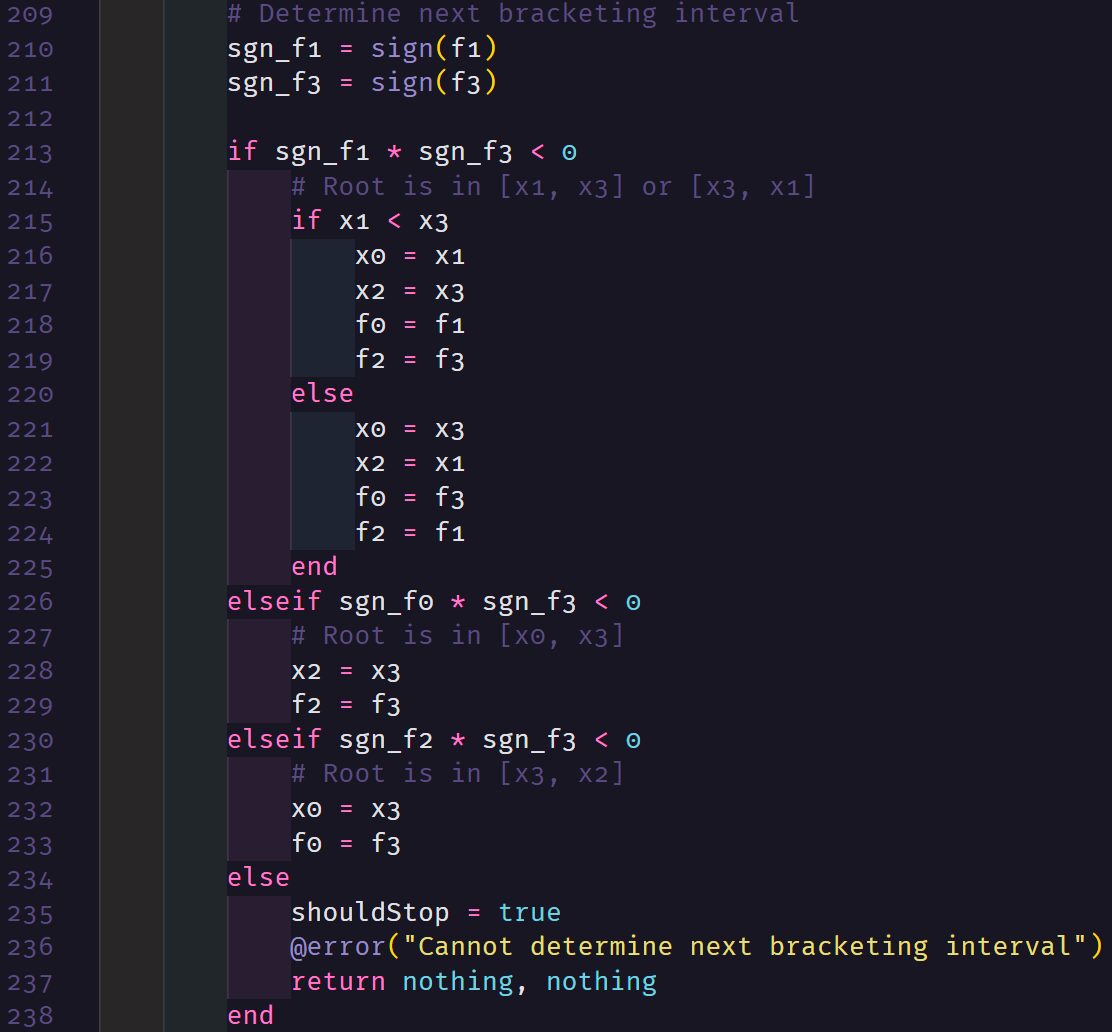
\includegraphics[width=0.95\textwidth]{figures/p05-3-codebase-5-ridders-search-part5.png}
    \caption{Ridders' function (part 5): Interval selection and convergence check.}
\end{figure}

\begin{figure}[H]
    \centering
    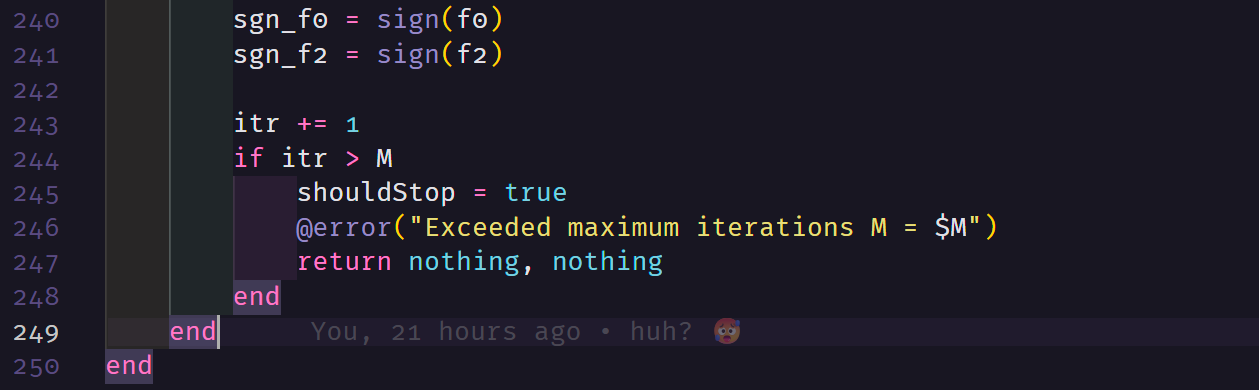
\includegraphics[width=0.95\textwidth]{figures/p05-3-codebase-6-ridders-search-part6.png}
    \caption{Ridders' function (part 6): Return result and exit.}
\end{figure}